\section{Injection Strategy}

The LUX collaboration agreed upon a three phase plan for a safe and successful tritium injection.  The first phase of this plan was a natural methane injection using the tritiated methane injection system for the purpose of determining the purification time constant in LUX.  The second phase of the plan was a small tritium injection (19 mBq) into LUX.  This small injection would highlight any potential problems before injecting a larger amount of tritium, and it would determine if any scaling factor was needed between the absolute injection activity and the observed injection activity.  Additionally, the small tritium injection would allow us to measure the fraction of tritium that goes into the fiducial volume.  Finally, the third phase of the plan was to use what we learned from the first two phases to safely inject a larger amount of tritium (15,000 events) for the purpose of measuring the ER rejection factor of LUX and cross-checking the NEST prediction of the ER band.

\subsection{Phase One}

During phase one 0.02 grams of natural methane were injected into LUX using the tritium injection system.  Purity samples from the detector were collected over the next few days, and a purification time constant of 5.90 $\pm$ 0.07 hours was determined using data collected with the LUX gas sampling system.

\begin{figure}[H]
\centering
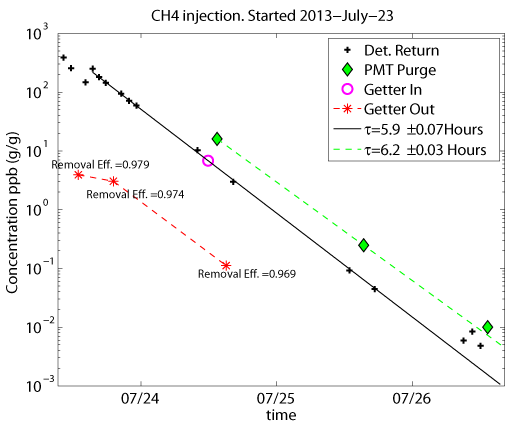
\includegraphics[scale=0.3]{CH4_injection.png}
\caption{First three days of the natural methane injection.  The discontinuity near the beginning of the data is due to a secondary natural methane injection.}
\label{fig:CH4Inject}
\end{figure}

\subsection{Phase Two and Three}

The first, smaller tritiated methane injection on Aug-08-2013 was done to confirm the purification model established by a natural methane purification campaign the previous week. An absolute activity of 20 mBq of tritiated methane was injected, while actively purifying. A purification time constant of 6.7 hours was observed, consistent with the natural methane purification rate measured by the sampling system. After a day of circulating through the getter the tritium decay had fallen below detectable amounts confirming the effective removal of the tritiated methane with the getter. On Aug-13-2013 a larger injection of 800 mBq was performed. The second injection produced 20,000 beta decay events in the LUX detector before being completely removed, 5000 of those events could be used the calibrate the ER band in the WIMP search region of 0-30 Phe (pulse area in photo electrons). 
Figure \ref{fig:Removal} shows the two tritium injections and the subsequent CH3T purification. Figure \ref{fig:Removal_2} shows the rate of events in the ER band before and after the tritium injection and removal. The CH3T was injected at the getter output but had passed through a special methane purifier to remove O2 and H2O or other impurities that could cause a degradation in election lifetime. The injections were performed with the getter in purify mode to maintain detector purity, as soon as the CH3T was injected is was immediately being removed.  The rate of tritiated methane removal was consistent with the removal of natural methane observed by the xenon sampling system which was used to first verify the removal of methane to $\rm 1/10^5$. Figure \ref{fig:Removal}.


\begin{figure}[H]\centering
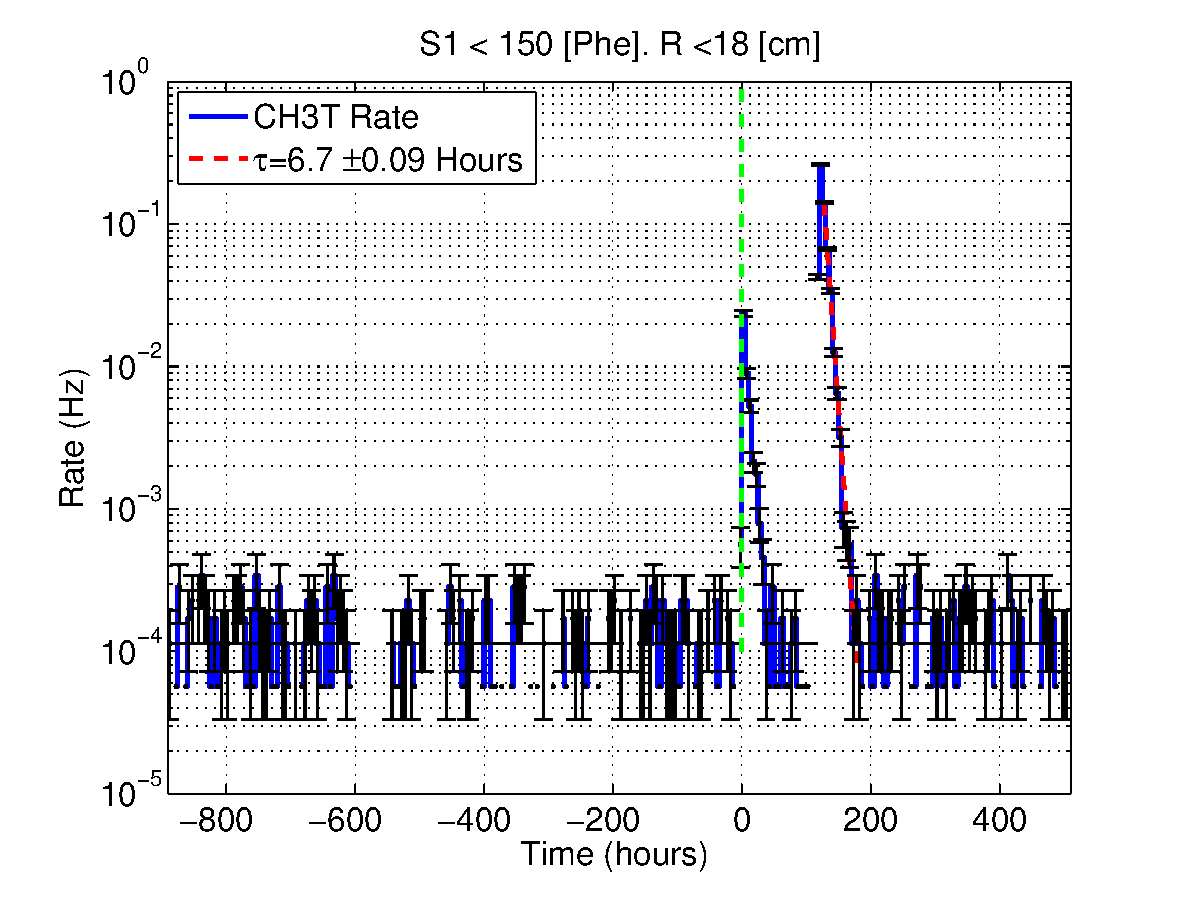
\includegraphics[width=80mm]{CH3T_Rate_fid_150_lux10_20130813T1120_note.eps}
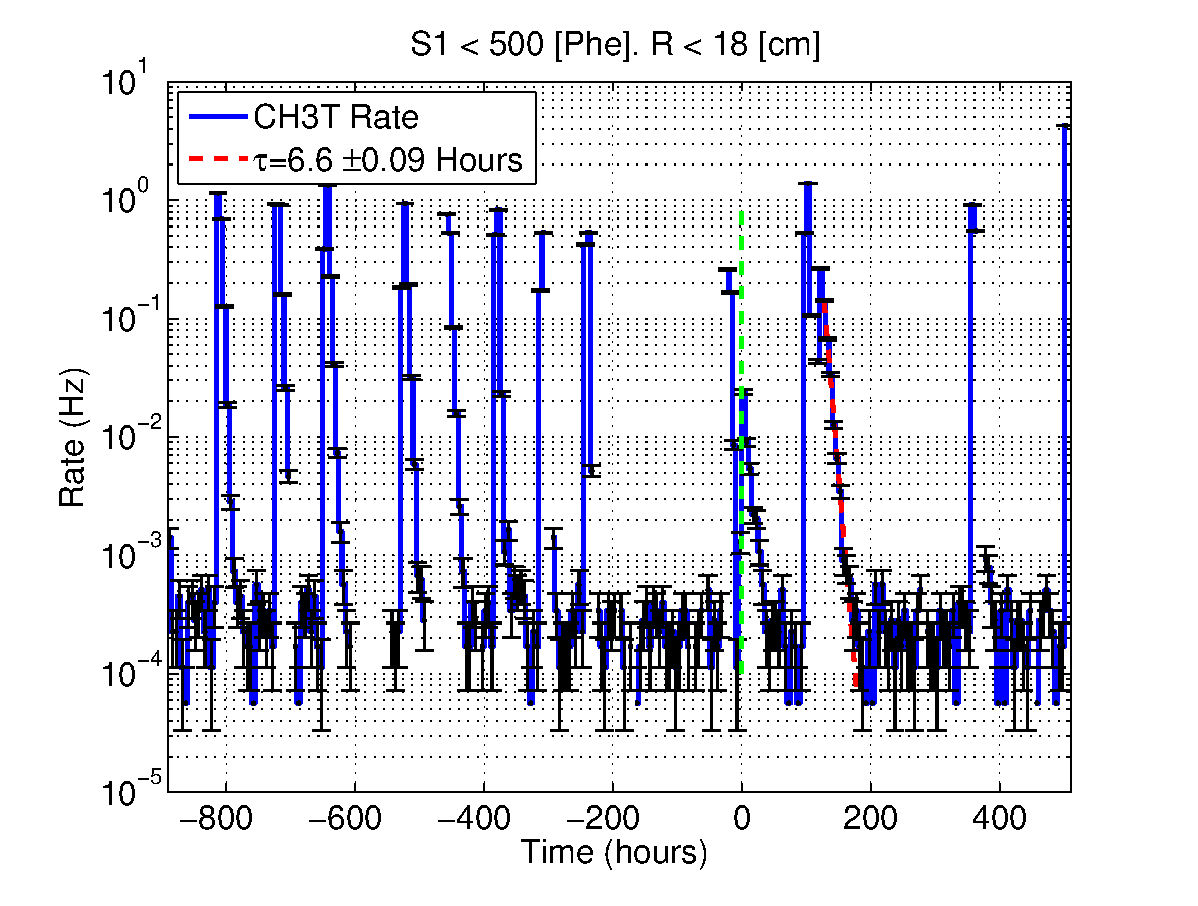
\includegraphics[width=80mm]{CH3T_Rate_fid_500_lux10_20130813T1120.eps}
\caption{Left: Rate of events in the WIMP search region over a two month window. The dashed, vertical green line represents the time of the fist tritiated methane injection. Right: The S1 threshold extended to 500 Phe to include rate spikes from the $\rm ^{83}Kr$ injections, used for detector calibration during the science run. }
\label{fig:Removal}
\end{figure}

\begin{figure}[H]\centering
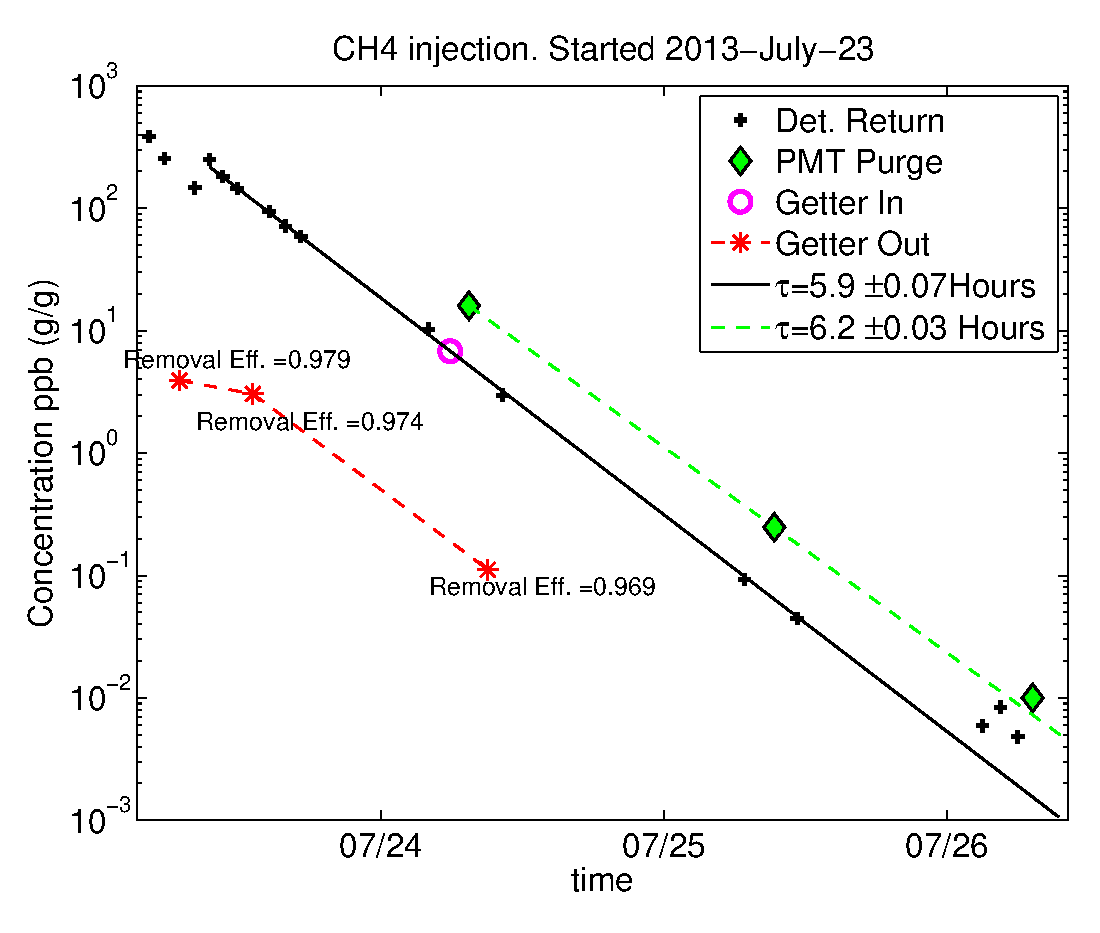
\includegraphics[width=80mm]{CH4_injection.eps}
\caption{Removal of natural methane observed by the xenon sampling system prior to the tritiated methane injections. }
\label{fig:Removal}
\end{figure}


\begin{figure}[H]\centering
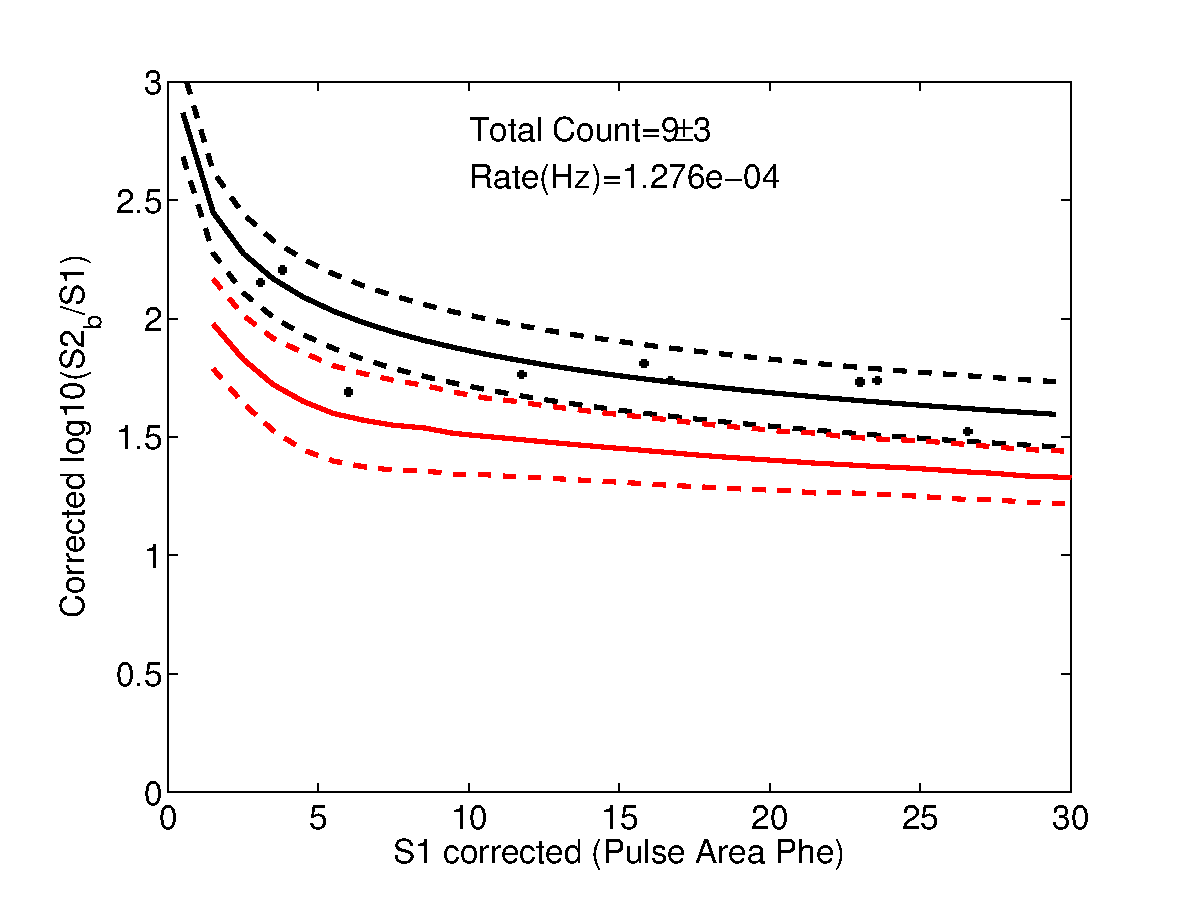
\includegraphics[width=80mm]{CH3T_fid_30_before_100_18_lux10_20130813T1120_cp05328_note.eps}
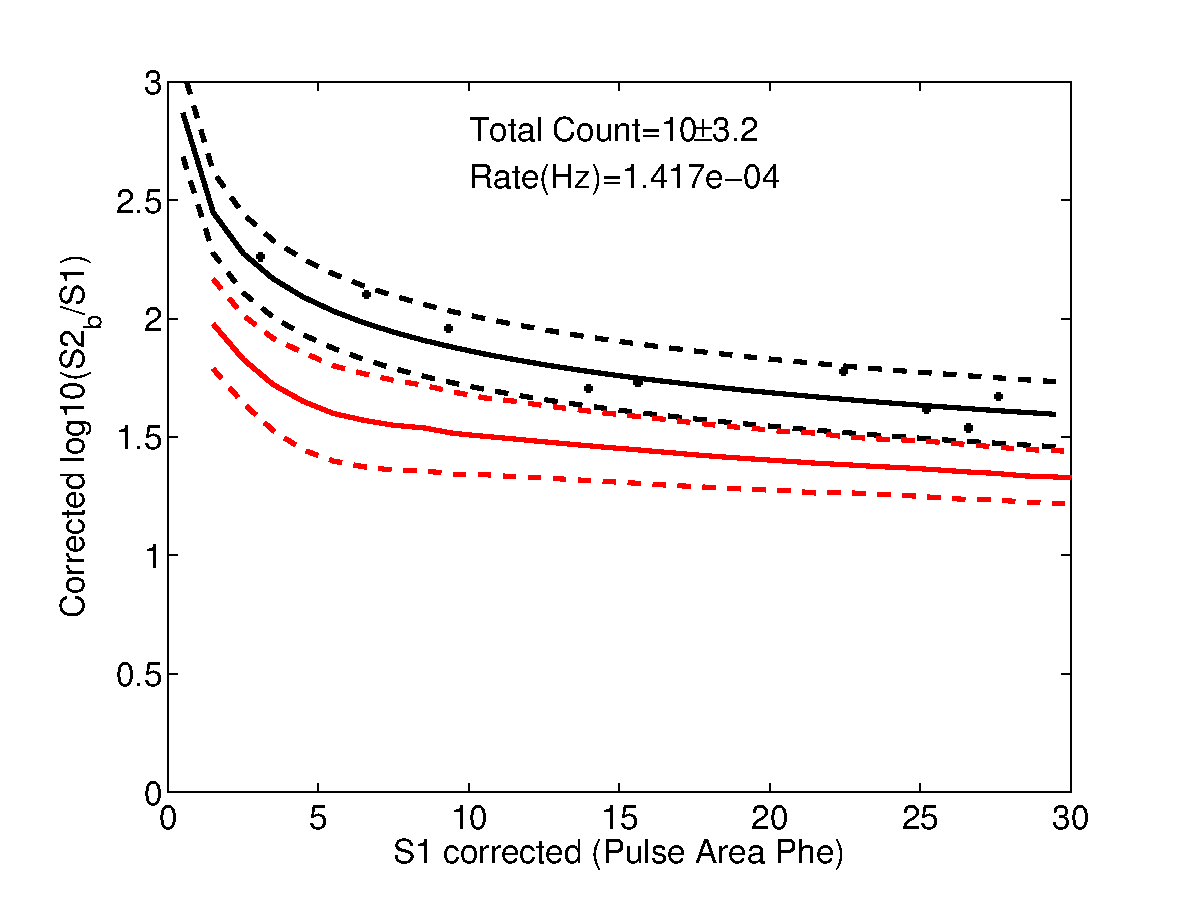
\includegraphics[width=80mm]{CH3T_fid_30_after_100_18_afterlux10_20130813T1120_cp05328_note.eps}
\caption{Left: 100 Hour time window in the WIMP search region before the tritiated methane injection. Right: 100 Hour time window in the WIMP search region after the purification of the tritiated methane. }
\label{fig:Removal_2}
\end{figure}

